%%%%%%%%%%%%%%%%%%%%%%%%%%%%%%%%%%%%%%%%%%%%%%%%%%%%%%%%%%%%%%%%%%%%
\section{Organization and Management}
\label{sec:fdgen-slow-cryo-org}
% sowjanya

%%%%%%%%%%%%%%%%%%%%%%%%%%%%%%%%%%%
\subsection{Slow Controls and Cryogenics Instrumentation Consortium Organization}
\label{sec:fdgen-slow-cryo-org-consortium}

% same in sp and dp

The organization of the CISC consortium is shown in
Fig.\ \ref{fig:gen-slow-cryo-org}. The CISC consortium board is
currently formed from institutional representatives from 17 institutes
as shown in Table \ref{tab:gen-slow-cryo-org}. The consortium leader
acts as the spokesperson for the consortium and is responsible for the
overall scientific program and management of the group. The technical
leader of the consortium is responsible for the project management for
the group.  Currently five working groups are envisioned in the
consortium (leaders to be appointed):


Cryogenics Systems gas analyzers, liquid level monitors and cryogenic internal piping; CFD simulations

Liquid Argon Instrumentation purity monitors, thermometers, cameras and light emitting system, and instrumentation test facility; feedthroughs; E-field simulations; Instrumentation precision studies; ProtoDUNE data analysis coordination efforts




\begin{description}
 \item[Cryogenics Systems] gas analyzers, liquid level
  monitors and cryogenic internal piping; CFD simulations
 \item[Liquid Argon Instrumentation] purity monitors, thermometers,
   cameras and light emitting system, and instrumentation test facility;
   feedthroughs; E-field simulations;
   Instrumentation precision studies;
   ProtoDUNE data analysis coordination efforts
 \item [Slow Controls Base Software and Databases]  Base software, alarms and archiving databases, and monitoring tools;
   variable naming convention and slow controls quantities
 \item [Slow Controls Detector System Interfaces] Signal processing software and hardware interfaces (e.g. power supplies);
   firmware; rack hardware and infrastructure   
 \item [Slow Controls External Interfaces] Interfaces with external detector systems (e.g. Cryogenics system, Beam, Facilities, DAQ)
\end{description}

\begin{dunefigure}[CISC consortium organization]{fig:gen-slow-cryo-org}
{CISC Consortium organizational chart}
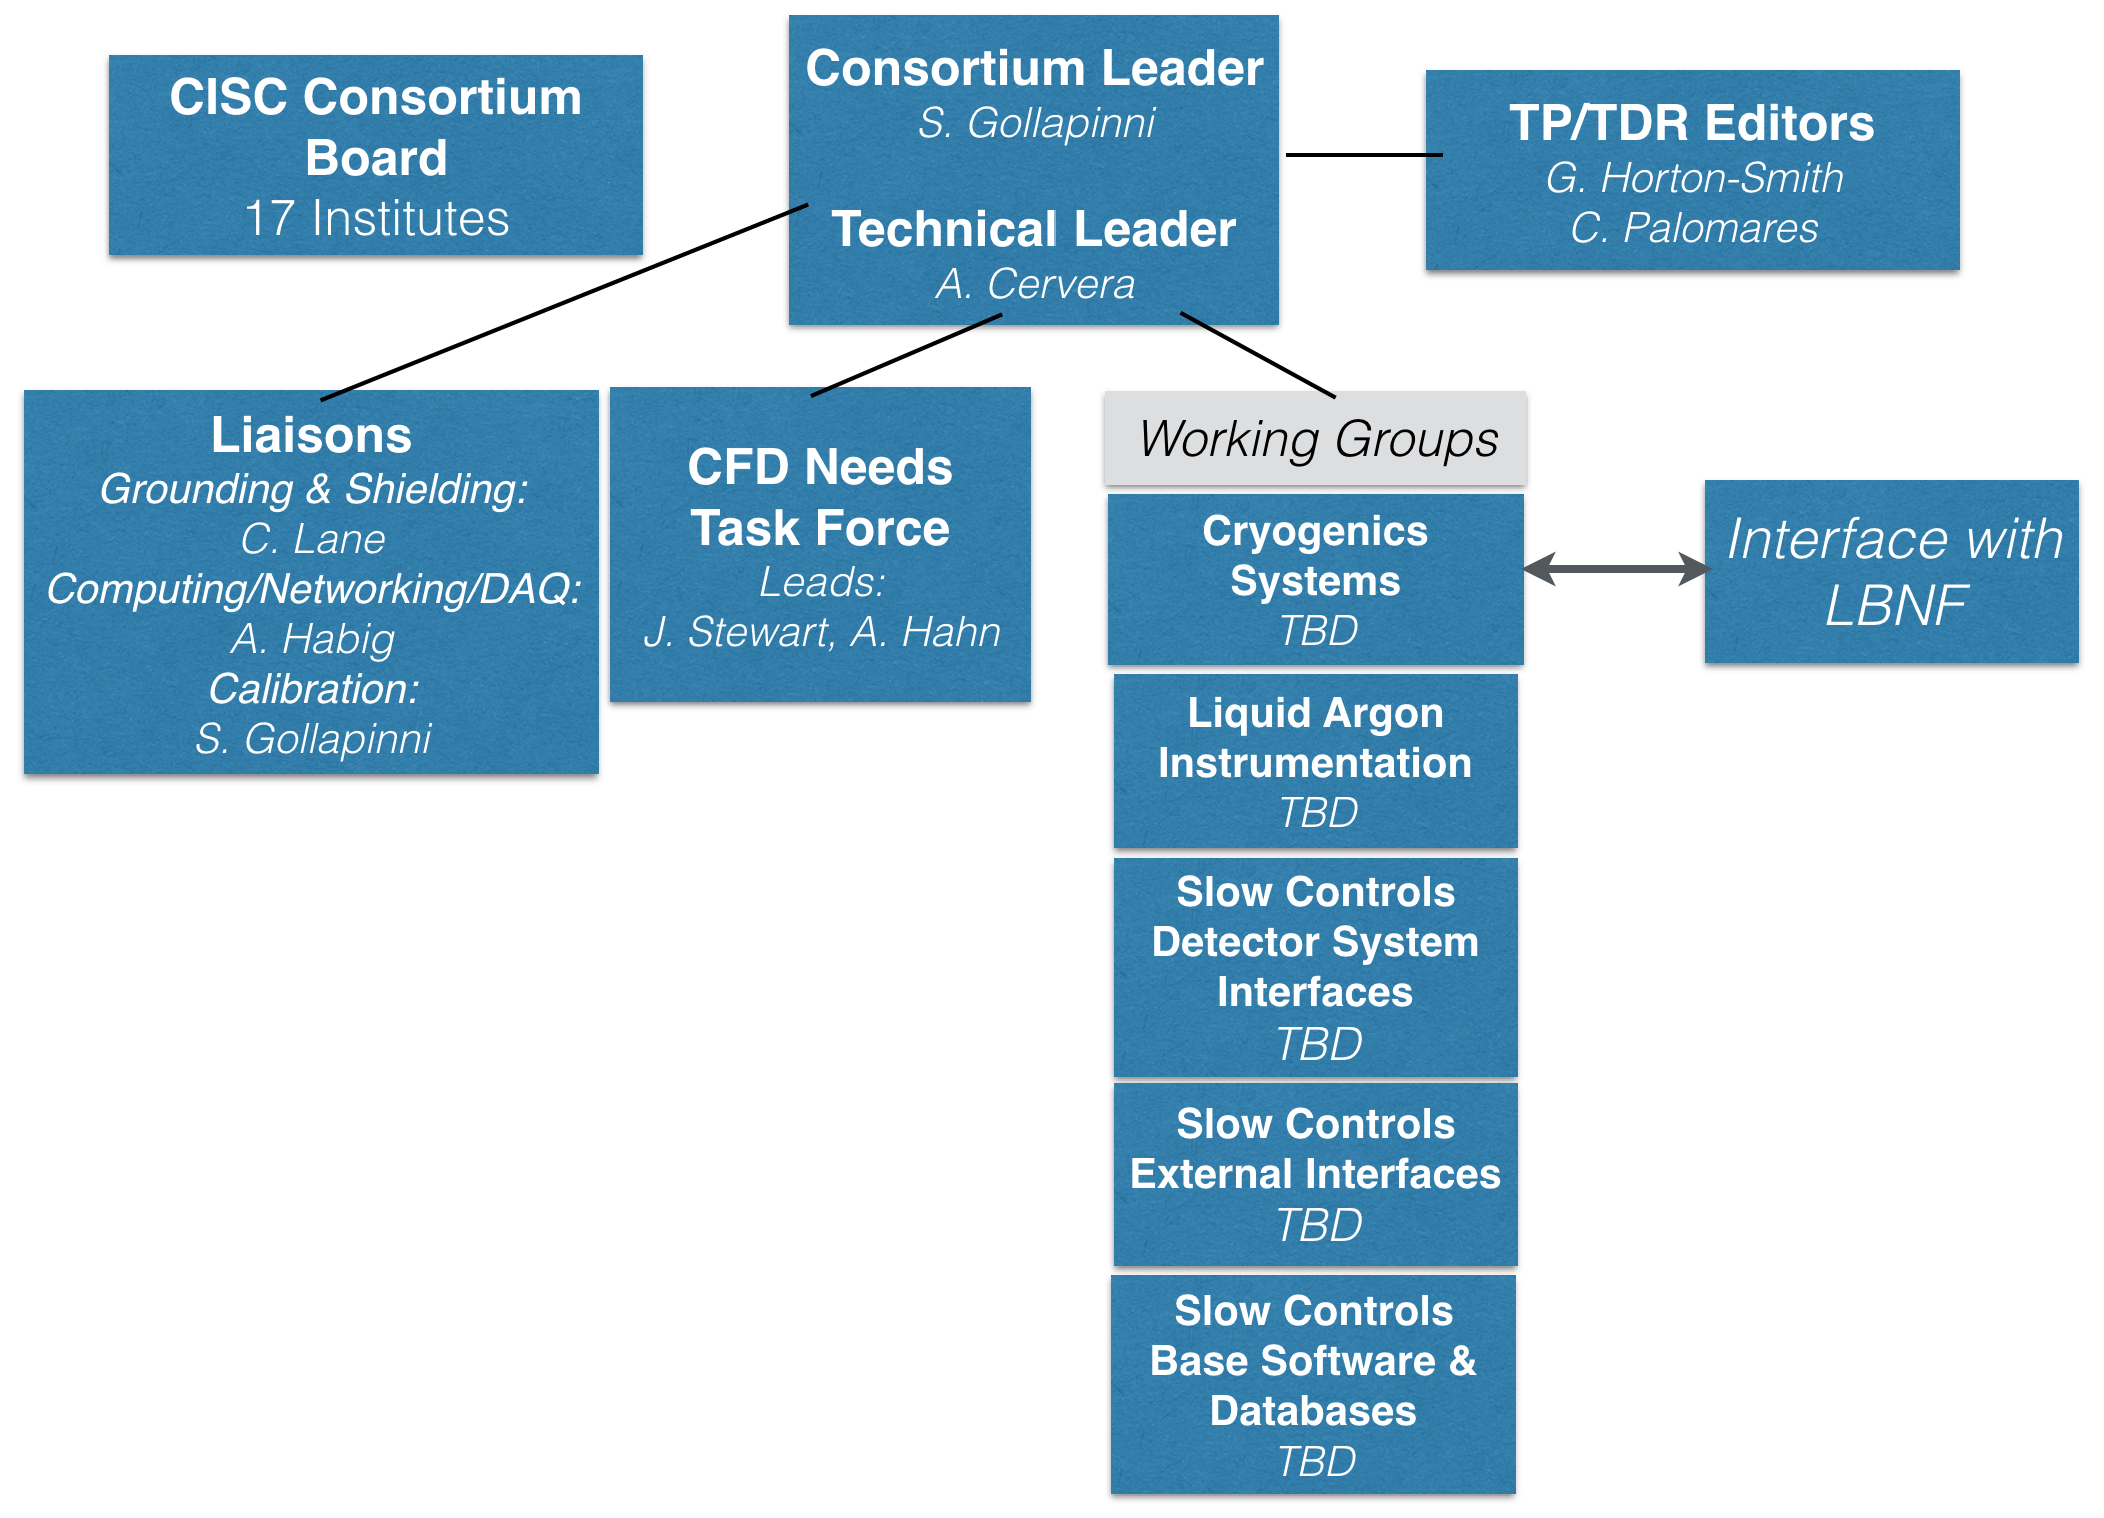
\includegraphics[width=0.7\textwidth]{cisc_org}
\end{dunefigure}

Additionally, since the CISC consortium broadly interfaces with other
groups, liaisons have been identified for various roles as listed in
Fig.\ \ref{fig:gen-slow-cryo-org}. A short-term focus group was
recently formed to understand the needs for cryogenic modeling for the
consortium. The Technical Proposal (TP) and Technical Design Report
(TDR) editors are responsible for the overall editing and delivery of
the TP/TDR documents to the collaboration. Currently members from new
institutes are added to the consortium based on consensus from the
consortium board members.

\begin{dunetable}
[CISC Consortium Institutions]
{p{0.3\textwidth}p{0.2\textwidth}p{0.3\textwidth}}
{tab:gen-slow-cryo-org}
{Current CISC Consortium Board Members and their institutional affiliations}
Member Institute  &  Country  &  Consortium Board Representative \\ \toprowrule
CIEMAT  &  Spain  &  Ines Gil Botella \\ \colhline
Instituto de Fisica Corpuscular  &  Spain  &  Anselmo Cervera \\ \colhline
University of Warwick  &  United Kingdom  &  Gary Barker \\ \colhline
University College London  &  United Kingdom  &  Mario Campanelli \\ \colhline
Argonne National Lab  &  USA  &  Jim Grudzinski  \\ \colhline
Brookhaven National Lab  &  USA  &  Jim Stewart \\ \colhline
University of California (Irvine)  &  USA  &  Jianming Bian \\ \colhline
Drexel University  &  USA  &  Charles Lane \\ \colhline
Fermi National Accelerator Lab  &  USA  &  Alan Hahn \\ \colhline
University of Hawaii  &  USA  &  Jelena Maricic \\ \colhline
University of Houston  &  USA  &  Andrew Renshaw \\ \colhline
Idaho State University  &  USA  &  Ed Tatar \\ \colhline
Kansas State University  &  USA  &  Glenn Horton-Smith \\ \colhline
University of Minnesota (Duluth)  &  USA  &  Alec Habig \\ \colhline
Notre Dame University  &  USA  &  John LoSecco \\ \colhline
University of Tennessee at Knoxville  &  USA  &  Sowjanya Gollapinni \\ \colhline
Virginia Tech &		USA	&	Camillo Mariani \\
\end{dunetable}


%%%%%%%%%%%%%%%%%%%%%%%%%%%%%%%%%%
\subsection{Planning Assumptions}
\label{sec:fdgen-slow-cryo-org-assmp}

The slow controls and cryogenic instrumentation will be a joint effort for single and dual phase.
A single slow controls system will be implemented to serve both dual and single phase.

Design and installation of cryogenic systems (gas analyzers, liquid level monitoring, internal piping) will be coordinated with LBNF, with the consortium providing resources, and effort and expertise provided by LBNF.
ProtoDUNE designs for liquid argon instrumentation (purity monitors, thermometers, cameras, test facility) will be the basis for DUNE designs. Design validation, testing, calibration, and performance will be evaluated through ProtoDUNE data.

% %%%%%%%%%%%%%%%%%%%%%%%%%%%%%%%%%%%
% The editors at meeting of 2/13 suggest that the WBS section should be deleted in the TP. Accordingly, I have commented it out.
% \subsection{WBS and Responsibilities}
% \label{sec:fdgen-slow-cryo-org-wbs}


%%%%%%%%%%%%%%%%%%%%%%%%%%%%%%%%%%
% The editors at meeting of 2/13 suggest that the TP need not have costing. Accordingly, I have renamed this section ``High-level Schedule''.
\subsection{High-level Schedule}
\label{sec:fdgen-slow-cryo-org-cs}

Table \ref{tab:fdgen-slow-cryo-schedule} shows key milestones on
the path to the Technical Design Report and CD-2.

\begin{dunetable}
[Key CISC Milestones leading to TDR]
{p{0.15\linewidth}p{0.60\linewidth}}
{tab:fdgen-slow-cryo-schedule}
{Key CISC Milestones leading to TDR.}   
Date & Milestone \\ \toprowrule
Dec.\ 2017  & Finalize Cryostat Instrumentation Feedthroughs \\ \colhline
Dec.\ 2017  & Develop a baseline conceptual design/layout for the internal cryogenic piping \\ \colhline
Mar.\ 2018 & Develop conceptual designs (including support structure) for all instrumentation devices \\ \colhline
Mar.\ 2018 & Define Slow controls hardware/software requirements and Layout \\ \colhline
Apr.\ 2018 & PrM design performance metrics for DUNE FD SP from ProtoDUNE-SP PrM tests in LAr \\ \colhline
May 2018   & Technical Proposal \\ \colhline
Aug.\ 2018   & Use ProtoDUNE-SP instrumentation/operations data to validate designs \\ \colhline
Nov.\ 2018  & Finish producing needed E-field and CFD simulations \\ \colhline
Dec.\ 2018  & Full design of the cryogenic instrumentation test facility \\ \colhline
Jan.\ 2019   & Develop a complete architectural design for Slow Controls \\ \colhline
Feb.\ 2019   & Finalize designs all instrumentation devices \\ \colhline
Apr.\ 2019 & Technical Design Report \\ \colhline
Oct.\ 2019 & CD-2 DOE Review \\
\end{dunetable}

